\chapter{Implementation extensions}\label{cha:software_new}
In the previous chapter, we found three important features that scikit-learn lacks in comparison to Weka's J48 implementation. In this chapter, we tackle the high priority pruning issue.

\section{New pruning functionality}
The most straightforward way to solve the pruning problem in scikit-learn is simply to implement an extension that provides this feature. This extension is simply a python package that can be downloaded and installed by anyone who already installed scikit-learn beforehand. We developed a new classifier called the \texttt{PruneableDecisionTreeClassifier} as the main component of such an extension. 

Instead of developing an extension, another option was to fork the complete current scikit-learn codebase and modified that in-place instead. The advantage of this approach is that pull requests can be made on Github to update the original codebase. However, in that case the code must adhere to a very strict contribution policy with requirements beyond the scope of this thesis. For example, scikit-learn must work perfectly with both Python 2.x and Python 3.x distributions. In this thesis we follow the way forward and only support Python 3.x. Additionally, keeping the code up to date involves regular merges with new scikit-learn code. This is not a problem with extensions built against a specific scikit-learn version (i.e., 0.19.1).

\subsection{Functional requirements}
The new class must enable tree pruning, but it must also function in a way highly similar to the original decision tree classifier in scikit-learn. This means it must:
\begin{itemize}
    \item have at least the same constructor arguments such as \texttt{criterion} and \texttt{splitter}
    \item support various pruning strategies
    \item have additional constructor arguments to specify the pruning method and related settings
    \item adhere to the basic classifier interface containing methods such as \texttt{fit}, \texttt{predict}, \texttt{predict\_proba} and \texttt{score}
    \item implement typical tree methods such as \texttt{apply} and \texttt{decision\_path}
    \item offer typical tree attributes such as \texttt{classes\_}, \texttt{feature\_importances\_} and \texttt{tree\_}
\end{itemize}

These requirements facilitate migrations to the new pruning-enabled decision tree classifier. Additionally, the new classifier remains compatible with existing scikit-learn tooling such as pipelines and grid searches.

From a software engineering perspective, meeting these requirements can be accomplished in two ways. Either make \texttt{PruneableDecisionTreeClassifier} inherit from \texttt{DecisionTreeClassifier} or implement the former using a decorator pattern. The result is the same, but the second option would require more boilerplate code. As such, the first option (inheritance) was chosen. The class diagram is shown in figure \ref{fig:classifier_classes}.

Adding pruning to an existing algorithm exclusively involves adding another step to the fitting process. In scikit-learn terms, this only requires an override of the \texttt{fit} method, while the other methods keep their existing implementation.

\begin{figure}[htp]
    \centering
    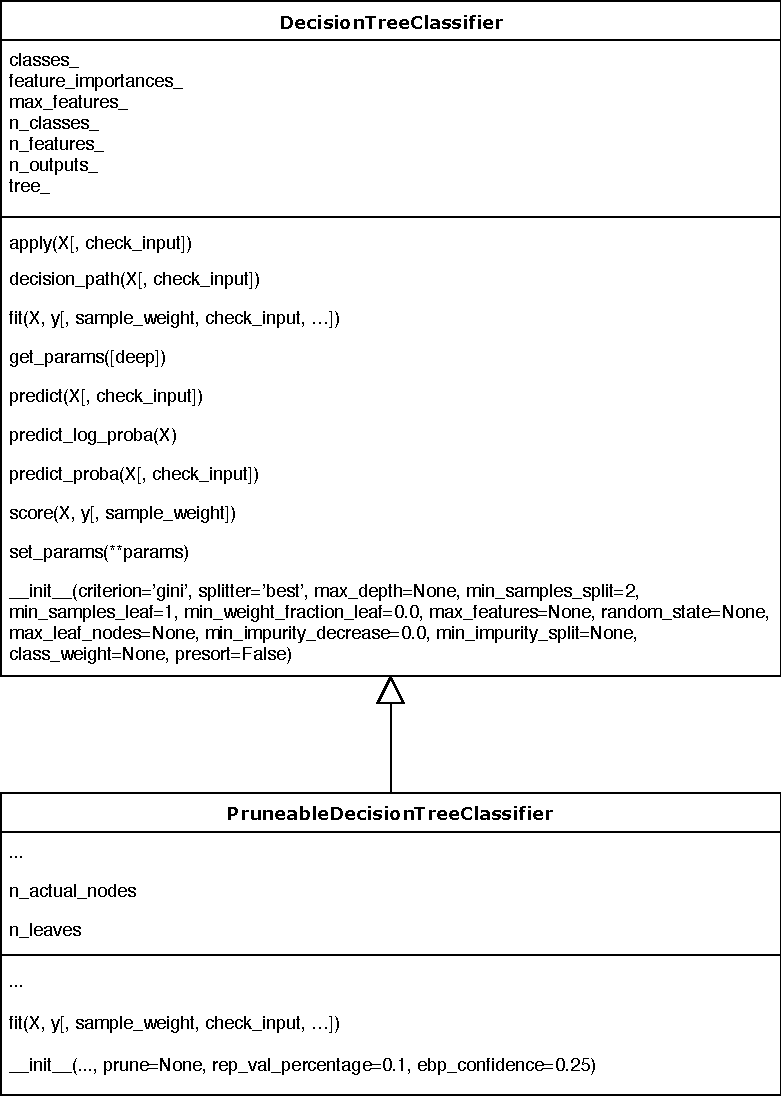
\includegraphics[width=\textwidth]{img/DecisionTreeClasses.pdf}
    \caption{Class diagram of decision tree classifiers.}%
    \label{fig:classifier_classes}
\end{figure}

\subsection{Pruning algorithms}
Various pruning strategies exist, as discussed in \autoref{cha:literature}. The goal is feature parity with J48, so both Reduced Error Pruning and Error Based Pruning are implemented. Additionally, the algorithm offers the option to disable pruning by setting the constructor argument \texttt{prune=None}. This way, users have no need to import the original classifier anymore.

Implementation-wise, the pruning logic has been isolated from the other tree logic in a separate class hierarchy. This is illustrated in figure \ref{fig:pruner_classes}. A base class \texttt{Pruner} is provided that contains all the tree operations that pruning algorithms will need such as \texttt{is\_leaf}, \texttt{to\_leaf} and \texttt{leaf\_prediction}. Two subclasses are also provided, the \texttt{ReducerErrorPruner} and the \texttt{ErrorBasedPruner}. Each one exposes a \texttt{prune} method. This way, supporting a new pruning strategy is as simple as adding a new class tot this hierarchy, instantiating it from the classifier and calling the \texttt{prune} method after the growth phase.

\begin{figure}[htp]
    \centering
    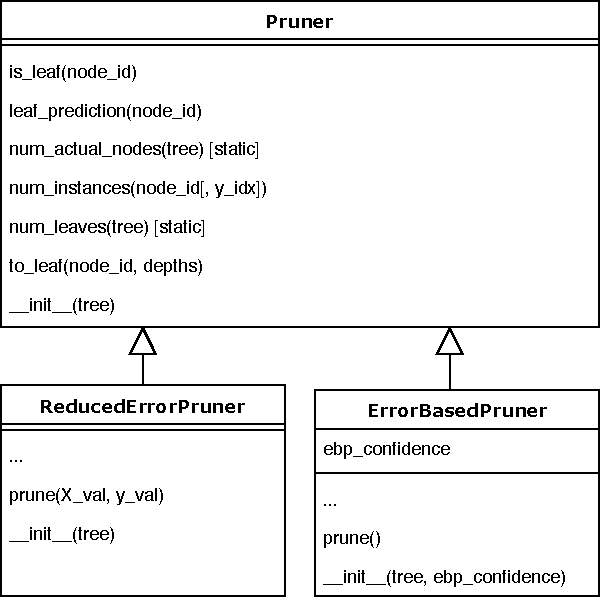
\includegraphics[width=0.8\textwidth]{img/PrunerClasses.pdf}
    \caption{Class diagram of pruners.}%
    \label{fig:pruner_classes}
\end{figure}

\subsubsection{Reduced Error Pruning}
Reduced Error Pruning is enabled by setting the constructor argument \texttt{prune='rep'}. It requires a separate validation set. There are two ways to deal with this problem. One, introduce two additional parameters to the fit method where the user can supply his own validation data (\texttt{X\_val}) and labels (\texttt{y\_val}). This maximizes the flexibility. However, it also places the burden of separating the original training set on the user. Worse, it breaks the classifier interface. Option two instead takes care of the separation internally using a stratified \texttt{test\_train\_split}. The user only has to provide the training set as usual, and also indicate which percentage of that set must be reserved for pruning via the \texttt{rep\_val\_percentage} argument. Because interface consistency is part of the functional requirements, option two was chosen. Weka's J48 contains a similar solution when this pruning strategy is used.

Once the two sets are separated, fitting can begin with the reduced training set using the existing implementation (i.e., the \texttt{fit} method of the base class). Afterwards, the \texttt{prune} method of a \texttt{ReducerErrorPruner} instance is called to simplify the tree.

\subsubsection{Error Based Pruning}
Error Based Pruning works similarly by setting the constructor argument \texttt{prune='ebp'}, but it does not require a validation set. Consequently, the training set provided by the user can be passed directly to the original \texttt{fit} method of the \texttt{DecisionTreeClassifier} base instance. Next, an instance of \texttt{ErrorBasedPruner} is created and its \texttt{prune} method is called with a confidence value that the user provided in the constructor of the new \texttt{PruneableDecisionTreeClassifier}. This confidence value is needed to calculate a statistical upper bound to the observed errors.

%performance: avoid for loops, maximize np calls
% -> cython not needed

%Example?
%pruning complexity O(...)

\section{Supporting tools}
\label{sec:csvimporter}
A lack of tree pruning algorithms was not the only problem of scikit-learn when compared to Weka's J48. It also has problems with categorical attributes and missing values. We will look at these problems in more detail later on. For now, some straightforward workarounds are implemented to make it possible to properly benchmark the new pruning solution. To that end, a \text{CsvImporter} class has been added to this extension that can parse arbitrary datasets. It adheres to the scikit-learn transformer interface, offering \texttt{fit}, \texttt{transform} and \texttt{fit\_transform} methods. The input is a file path to a Comma Separated Value (CSV) file, and the output is an \texttt{X, y} pair ready for consumption by tree induction algorithms\footnote{Strictly speaking, the \texttt{fit\_transform} method can only return the data \texttt{X} but not the labels \texttt{y} due to interface restrictions. Instead, \texttt{fit\_transform\_both} was introduced as a workaround.}.

TODO example

NumPy and SciPy --- the base libraries that scikit-learn is built upon --- already offer similar methods, but they are not suitable for our use cases. For example, SciPy offers a method to parse Weka's Attribute-Relation File Format (ARFF). This format contains valuable information, such as whether a variable is numerical or categorical (including the domain). This information is returned by the method as a structured array that keeps data type information per column instead of one data type for all values. Unfortunately these special arrays are not compatible with most machine learning algorithms. Numpy on the other hand offers a method to read plain text files such as CSV files into regular arrays. However, this function is known in the SciPy community to be unreliable and it also lacks modern features that libraries such as Pandas have available.

Our new solution is based on Pandas. Since it starts from plain CSV files instead of ARFF files, it has to infer the data types of each column based on the contents. Next, it deals with missing values rather abruptly by deleting all incomplete observations. A warning is triggered if a given threshold of data loss is surpassed. Scikit-learn offers more advanced methods of dealing with missing values independent of the machine learning algorithm used in the \texttt{impute} submodule~\cite{imputation}. The simple imputer only looks at other values in the same column to guess the value of a missing entry, which is also a very blunt method. The advanced version on the other hand makes various assumptions about the distribution of the data that cannot be guaranteed. These methods can be interesting for specific datasets, but our solution must work across a wide range of datasets. Consequently, the straightforward dropping strategy remains in use until a decision tree specific algorithm is implemented to alleviate this problem.

In the next phase, the class column --- as indicated by the user --- is separated from the rest of the data and the labels are encoded to integers in the range $[0, n\_classes - 1]$. The original values are also preserved to enable an inverse transformation after classification if needed. 

Finally, in the rest of the data, values of categorical attributes are encoded in a one-hot fashion to avoid creating an implicit ordering as discussed earlier in \autoref{sssec:cat_num_attr}. At this point the dataset contains no more missing or categorical values. It is ready to be used in decision tree induction algorithms.

%TODO class diagram? https://www.draw.io

\section{Limitations}
%no multi label, multi output
%internal data structures

\section{Challenges}
% cython
% tooling/testing/docs takes long time
% tooling limits potential of trees (labelencoder, pipeline, gridsearchcv)
% edge cases

\section{Result}
The resulting implementation is publicly hosted at \url{https://github.com/vhsven/vhsven-sklearn}. Comprehensive documentation and several examples are all available at \url{https://vhsven.github.io/vhsven-sklearn}. Check out the three examples concerning decision surfaces to get an intuitive feel of what the effect of each pruning method is.

%TODO add images here? also of original and pruned tree